% !TeX root = ./jvk-blatt1.tex

\excercise{DemoTask und UI}
\label{ex3}

\begin{enumerate}
    \item Nun wollen wir - wie in Aufgabe 1 \ref{ex1b} gezeigt - ein Spiel starten, indem wir den Code in der \lstinline{Main}-Klasse anpassen.\\
    Dieses Mal wollen wir die übergebenen Parameter allerdings etwas anpassen und das Spiel nur mit einer \lstinline{DemoTask} und noch ohne den \lstinline{DemoTaskVerifier} starten.\\
	Dafür erzeugen wir zunächst eine neue \lstinline{Game}-Instanz, indem wir den folgenden Code in die \lstinline{main()}-Methode einfügen:

    \begin{lstlisting}
		Game myGame = new Game("Hello World", new DemoTask());
    \end{lstlisting}

    Das Spiel kann gestartet werden, wenn du nun auf der Variable \lstinline{myGame} die Operation \lstinline{run()} aufrufst:

    \begin{lstlisting}
	myGame.run();
    \end{lstlisting}

    Starte das Programm nun in Eclipse, wie Du es schon in \ref{ex1} getan hast.

    \vspace{5mm}

    \item In der vorherigen Teilaufgabe haben wir bereits \lstinline{"Hello World"} und ein neues \lstinline{DemoTask}-Objekt an ein \lstinline{Game} übergeben.\\
    Nun wollen wir noch, wie ganz am Anfang, ein DemoTaskVerifier Objekt übergeben:

    \begin{lstlisting}
		Game myGame = new Game("Hello World", new DemoTask(), new DemoTaskVerifier());
    \end{lstlisting}

        Was hat sich nun im Spielfenster verändert?\\
        Finde den \q{Task Status} Tab in der Game-UI und drücke den Refresh Button.

\end{enumerate}


\begin{Infobox}[Der Refresh Button]
    Wenn du überprüfen willst, ob du deine Aufgabe erledigt hast, musst du den \fbox{Task Status} Tab unter dem Spielfeld öffnen und dann auf \fbox{Refresh} klicken.\\

    Wichtig: Der Task Status aktualisiert sich nicht automatisch. Du musst also immer selber aktualisieren.
\end{Infobox}


\begin{enumerate}\setcounter{enumi}{2}

    \item Finde sowohl im Spiel als auch in Eclipse die Konsole. Dies ist ein Feld in dem Text ausgegeben wird:
    \begin{center}
        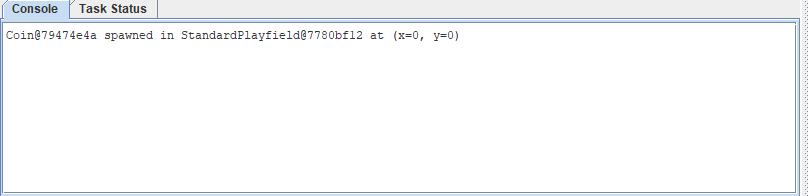
\includegraphics[width=\linewidth]{./figures/console.PNG}
    \end{center}

    In der Konsole siehst du, dass eine Münze (\texttt{Coin}) gespawnt (erzeugt) wurde.
    Finde die Koordinaten des Feldes, auf welchem die Münze gespawnt wurde.

    \item Nun suche nach der Stelle im Code in der Klasse \lstinline{DemoTask}, in dem die erste Münze erzeugt wird.\\
    \label{ex3d}
    Kleiner Tipp:
    Wenn du \fbox{Strg} drückst während du auf einen Klassennamen oder einen Operationsnamen im Code klickst, öffnet Eclipse die entsprechende Java-Datei wo sich diese Operation oder Klasse befindet.\\
    Alternativ kannst du über den PackageExplorer in das Paket\\\texttt{de.unistuttagrt.informatik.fius.jvk.tasks} navigieren und dort die Datei \texttt{DemoTask.java} mit einem Doppelklick öffnen.
\end{enumerate}
